\chapter{HLA - Lightly cluttered room}
\label{app:hla}
\begin{figure}[H]
\centering
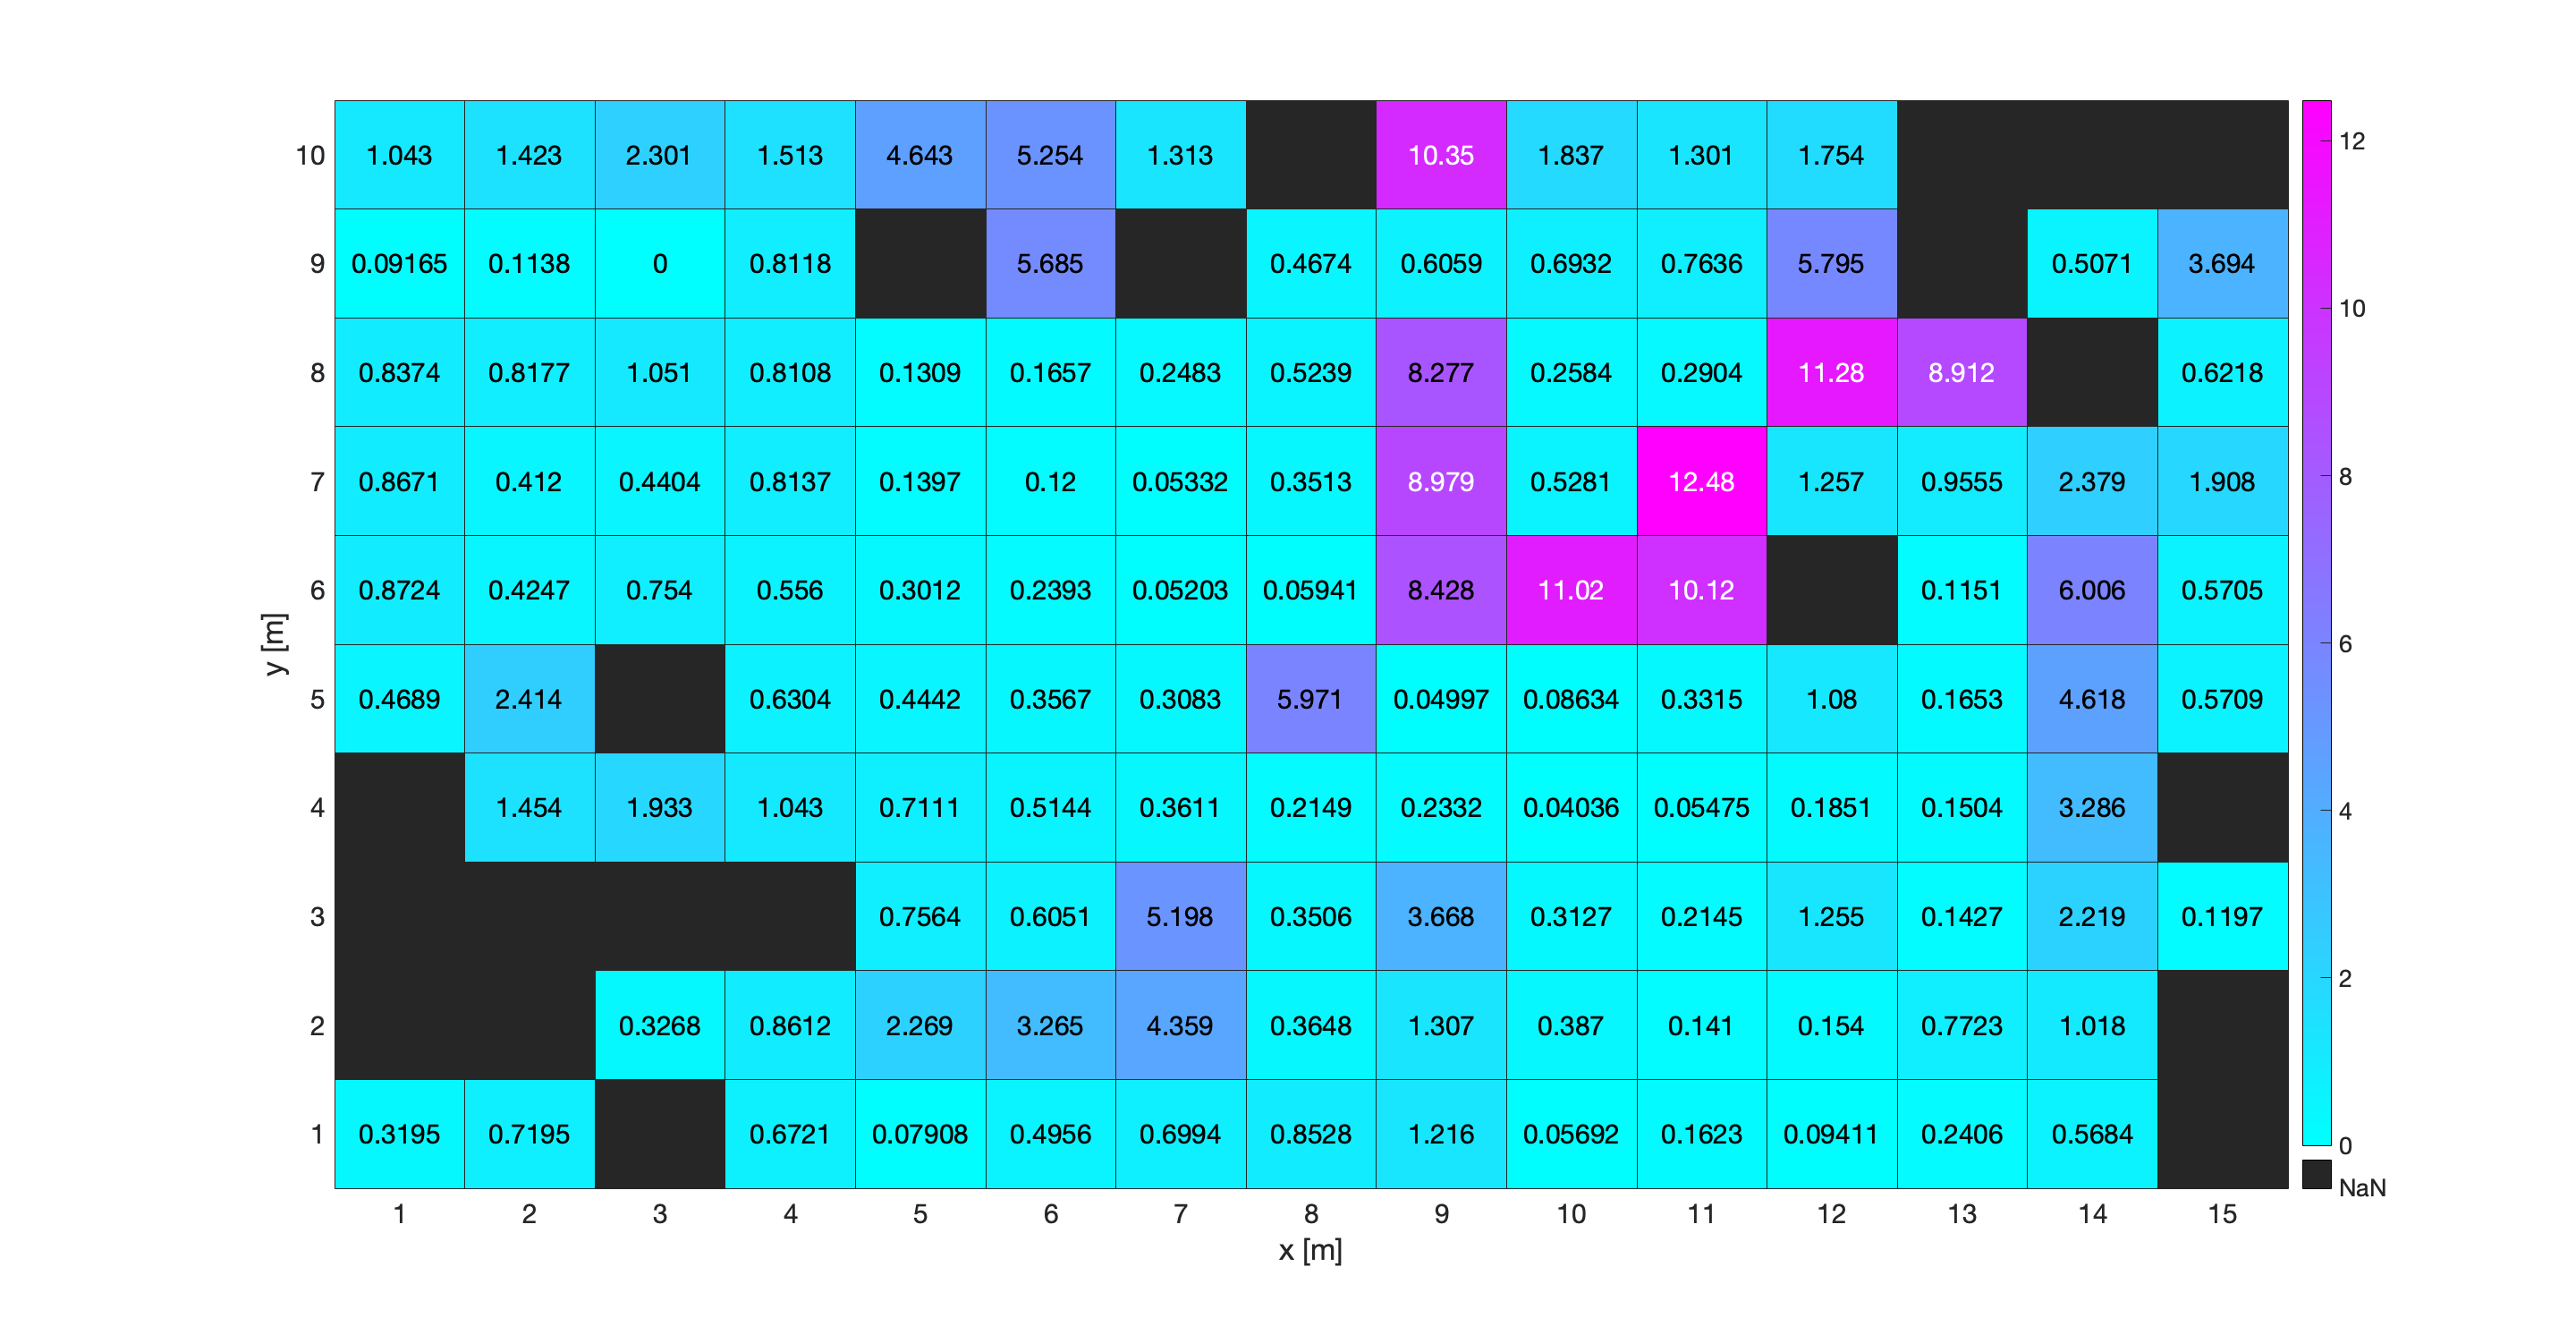
\includegraphics[width=.9\linewidth]{Images/hla_images/hla_anchor_(3_9)_clut.png}
\caption{Anchor located at (3, 9).}
\end{figure}

\begin{figure}[H]
\centering
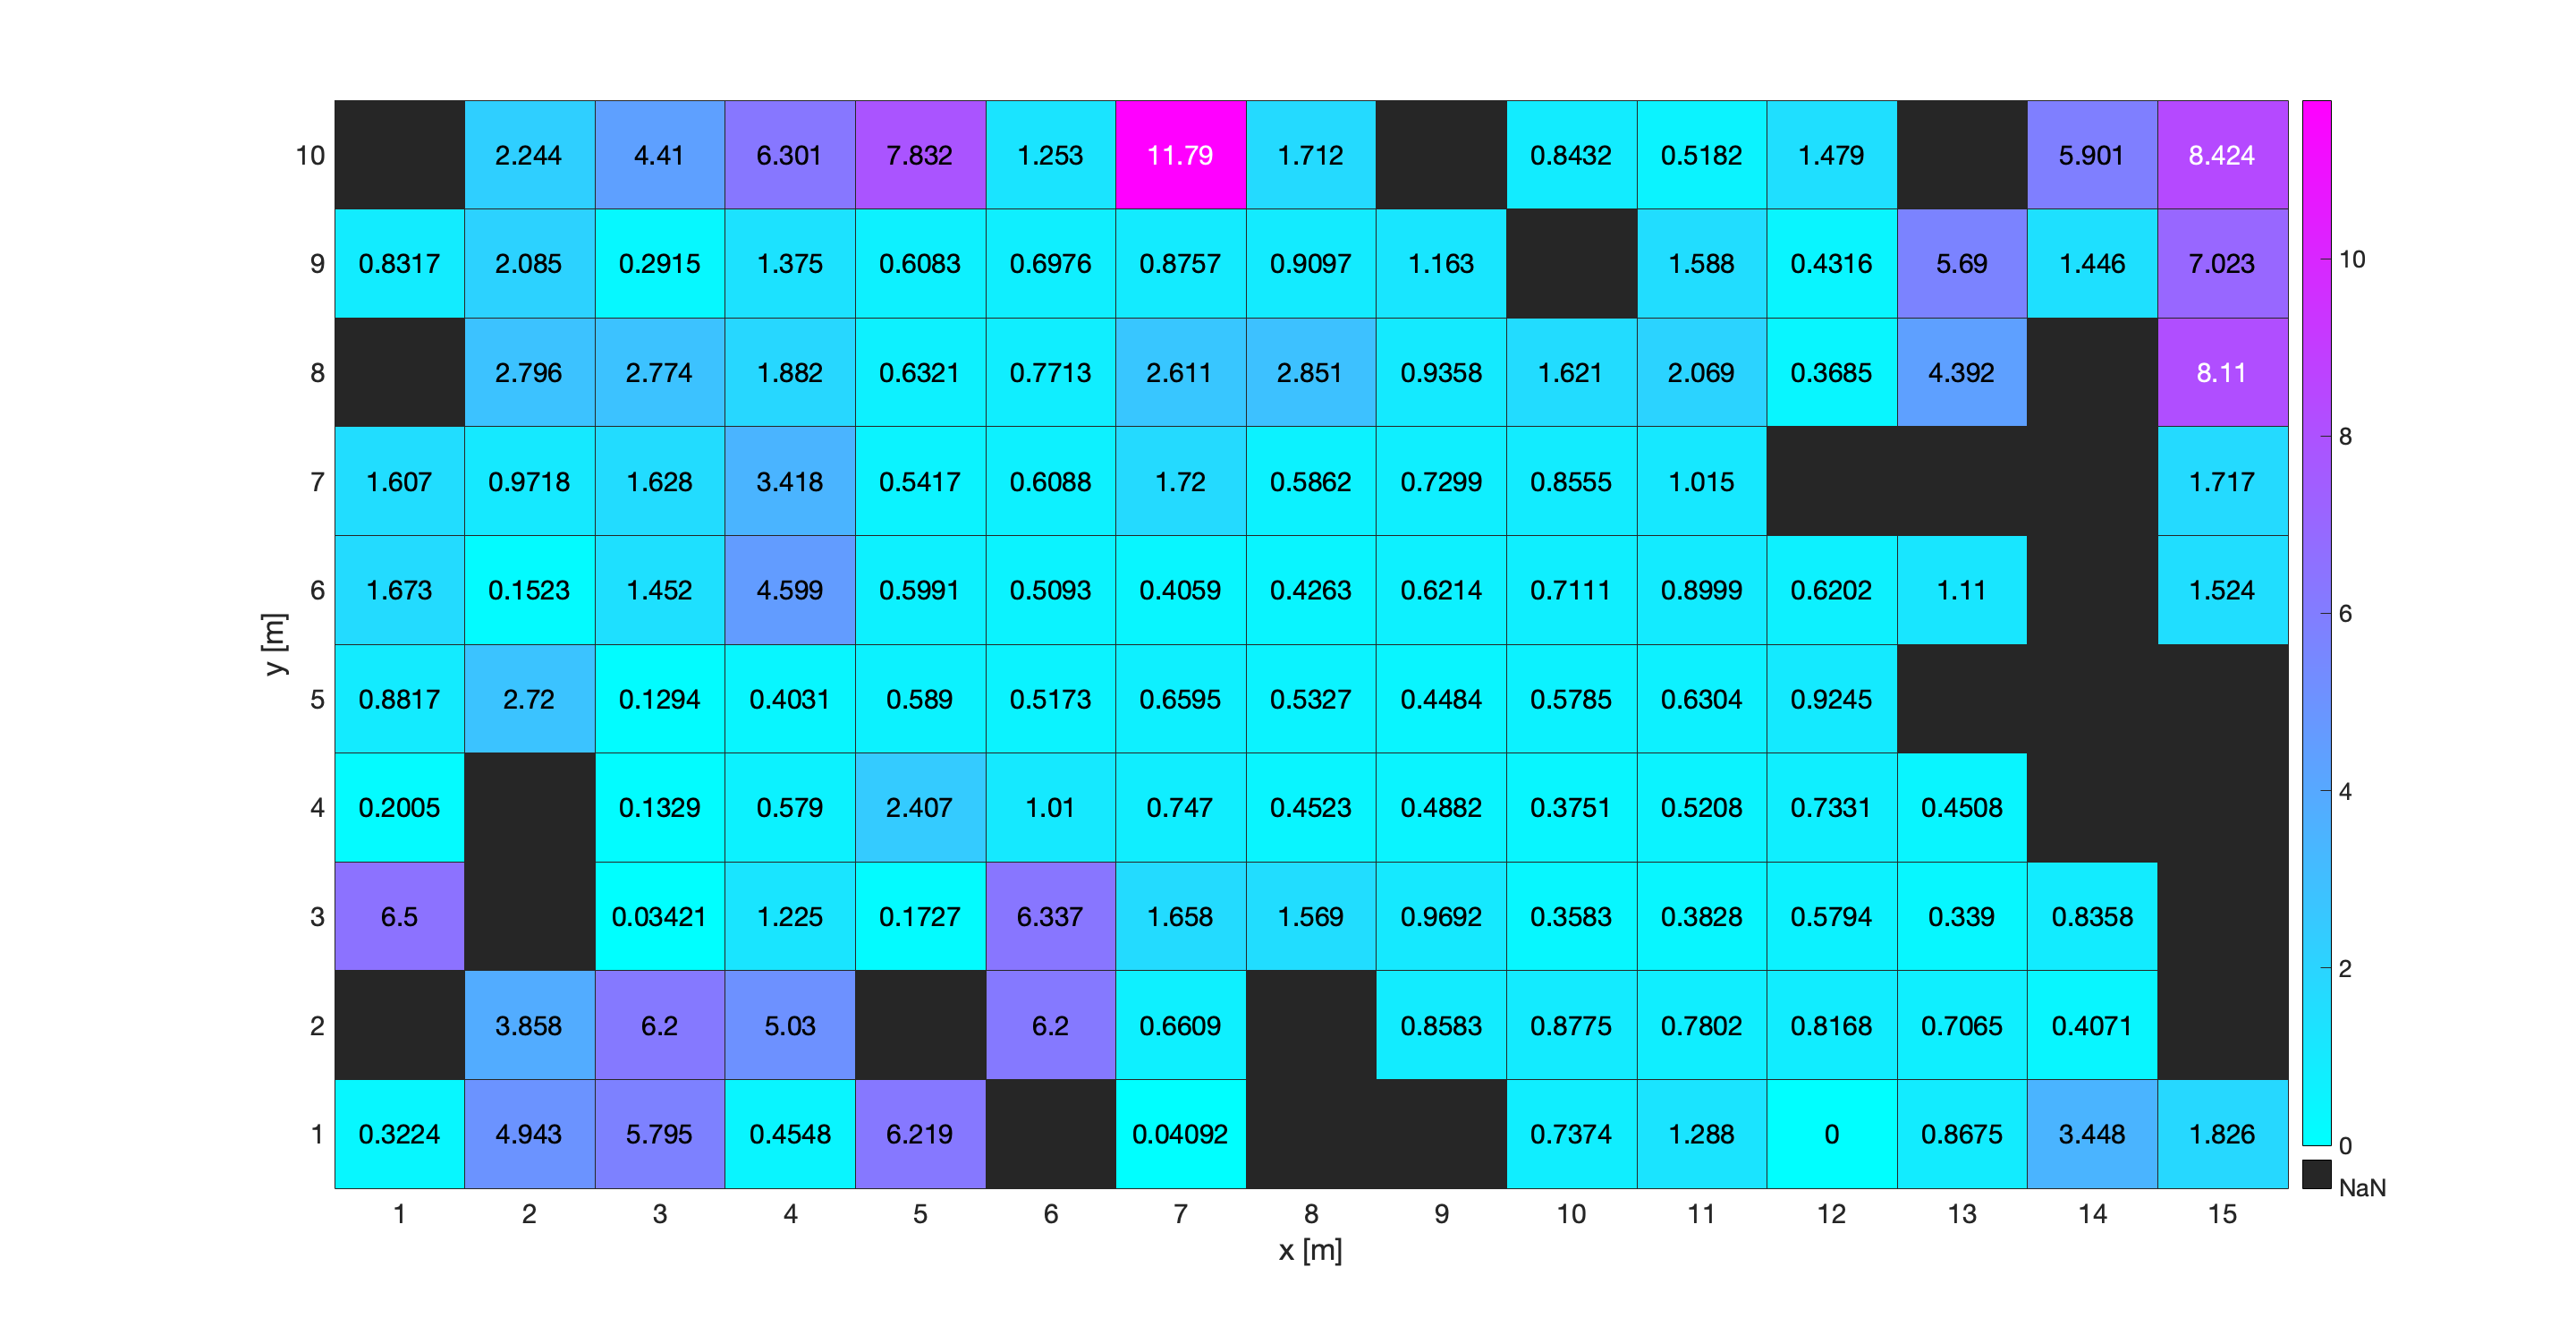
\includegraphics[width=.9\linewidth]{Images/hla_images/hla_anchor_(12_1)_clut.png}
\caption{Anchor located at (12, 1).}
\end{figure}

\begin{figure}[H]
\centering
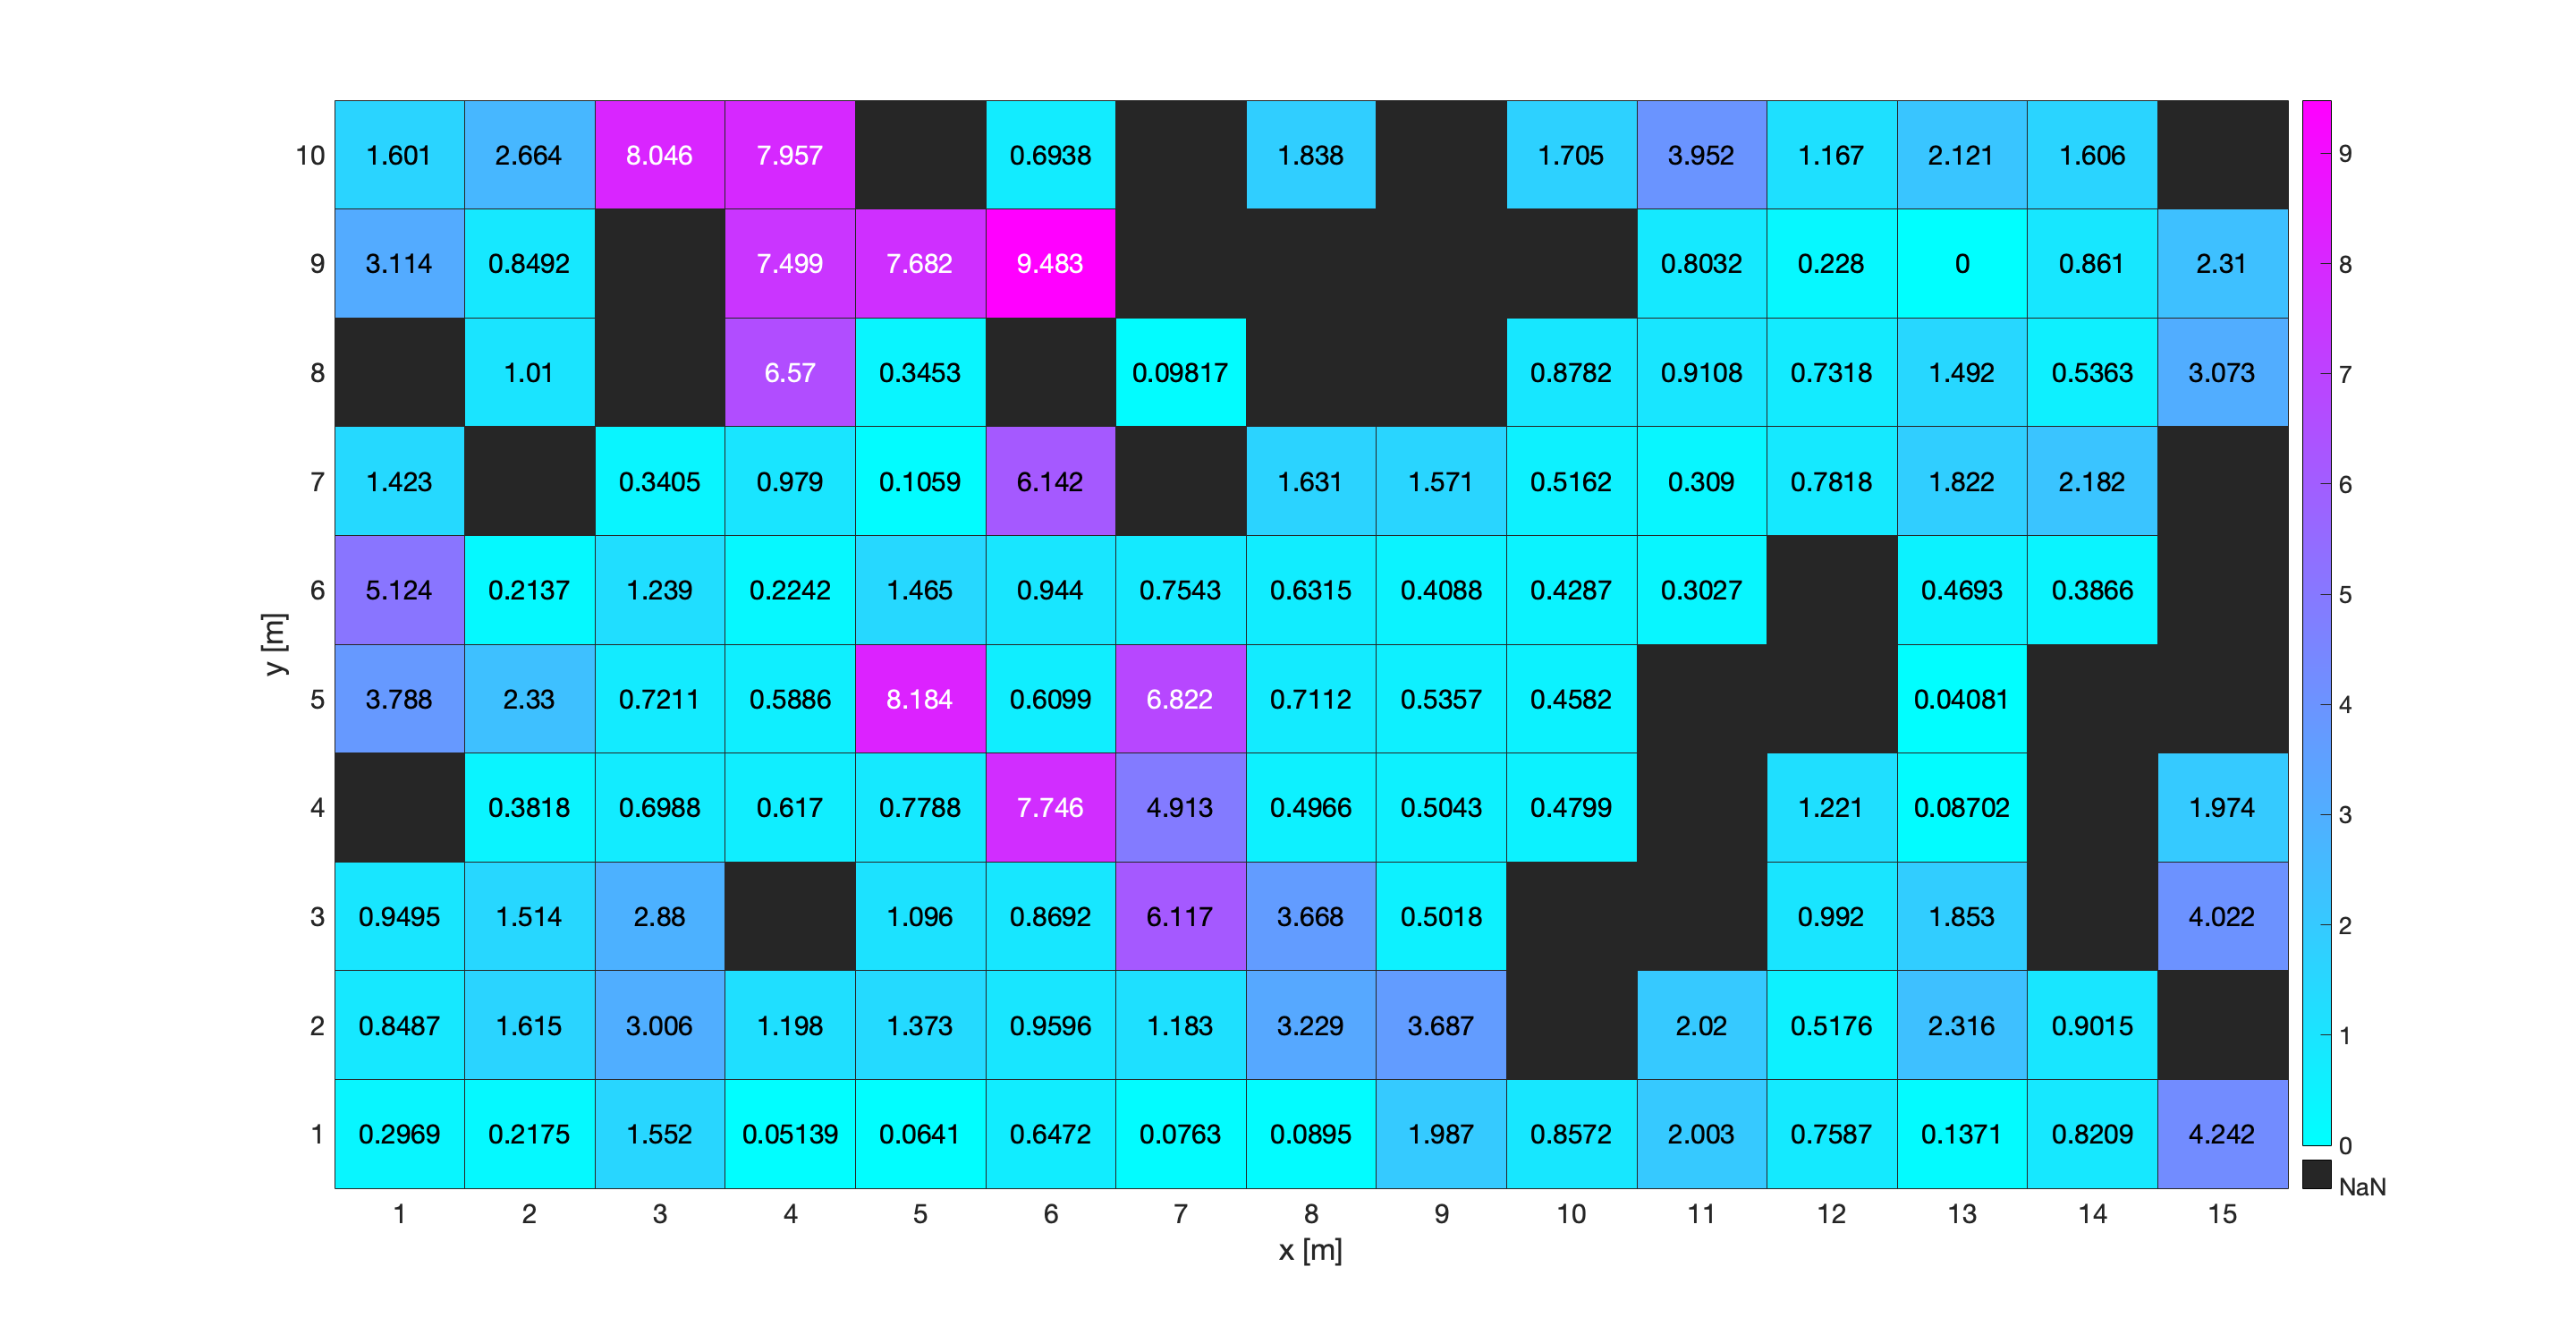
\includegraphics[width=.9\linewidth]{Images/hla_images/hla_anchor_(13_9)_clut.png}
\caption{Anchor located at (13, 9).}
\end{figure}

\begin{figure}[H]
\centering
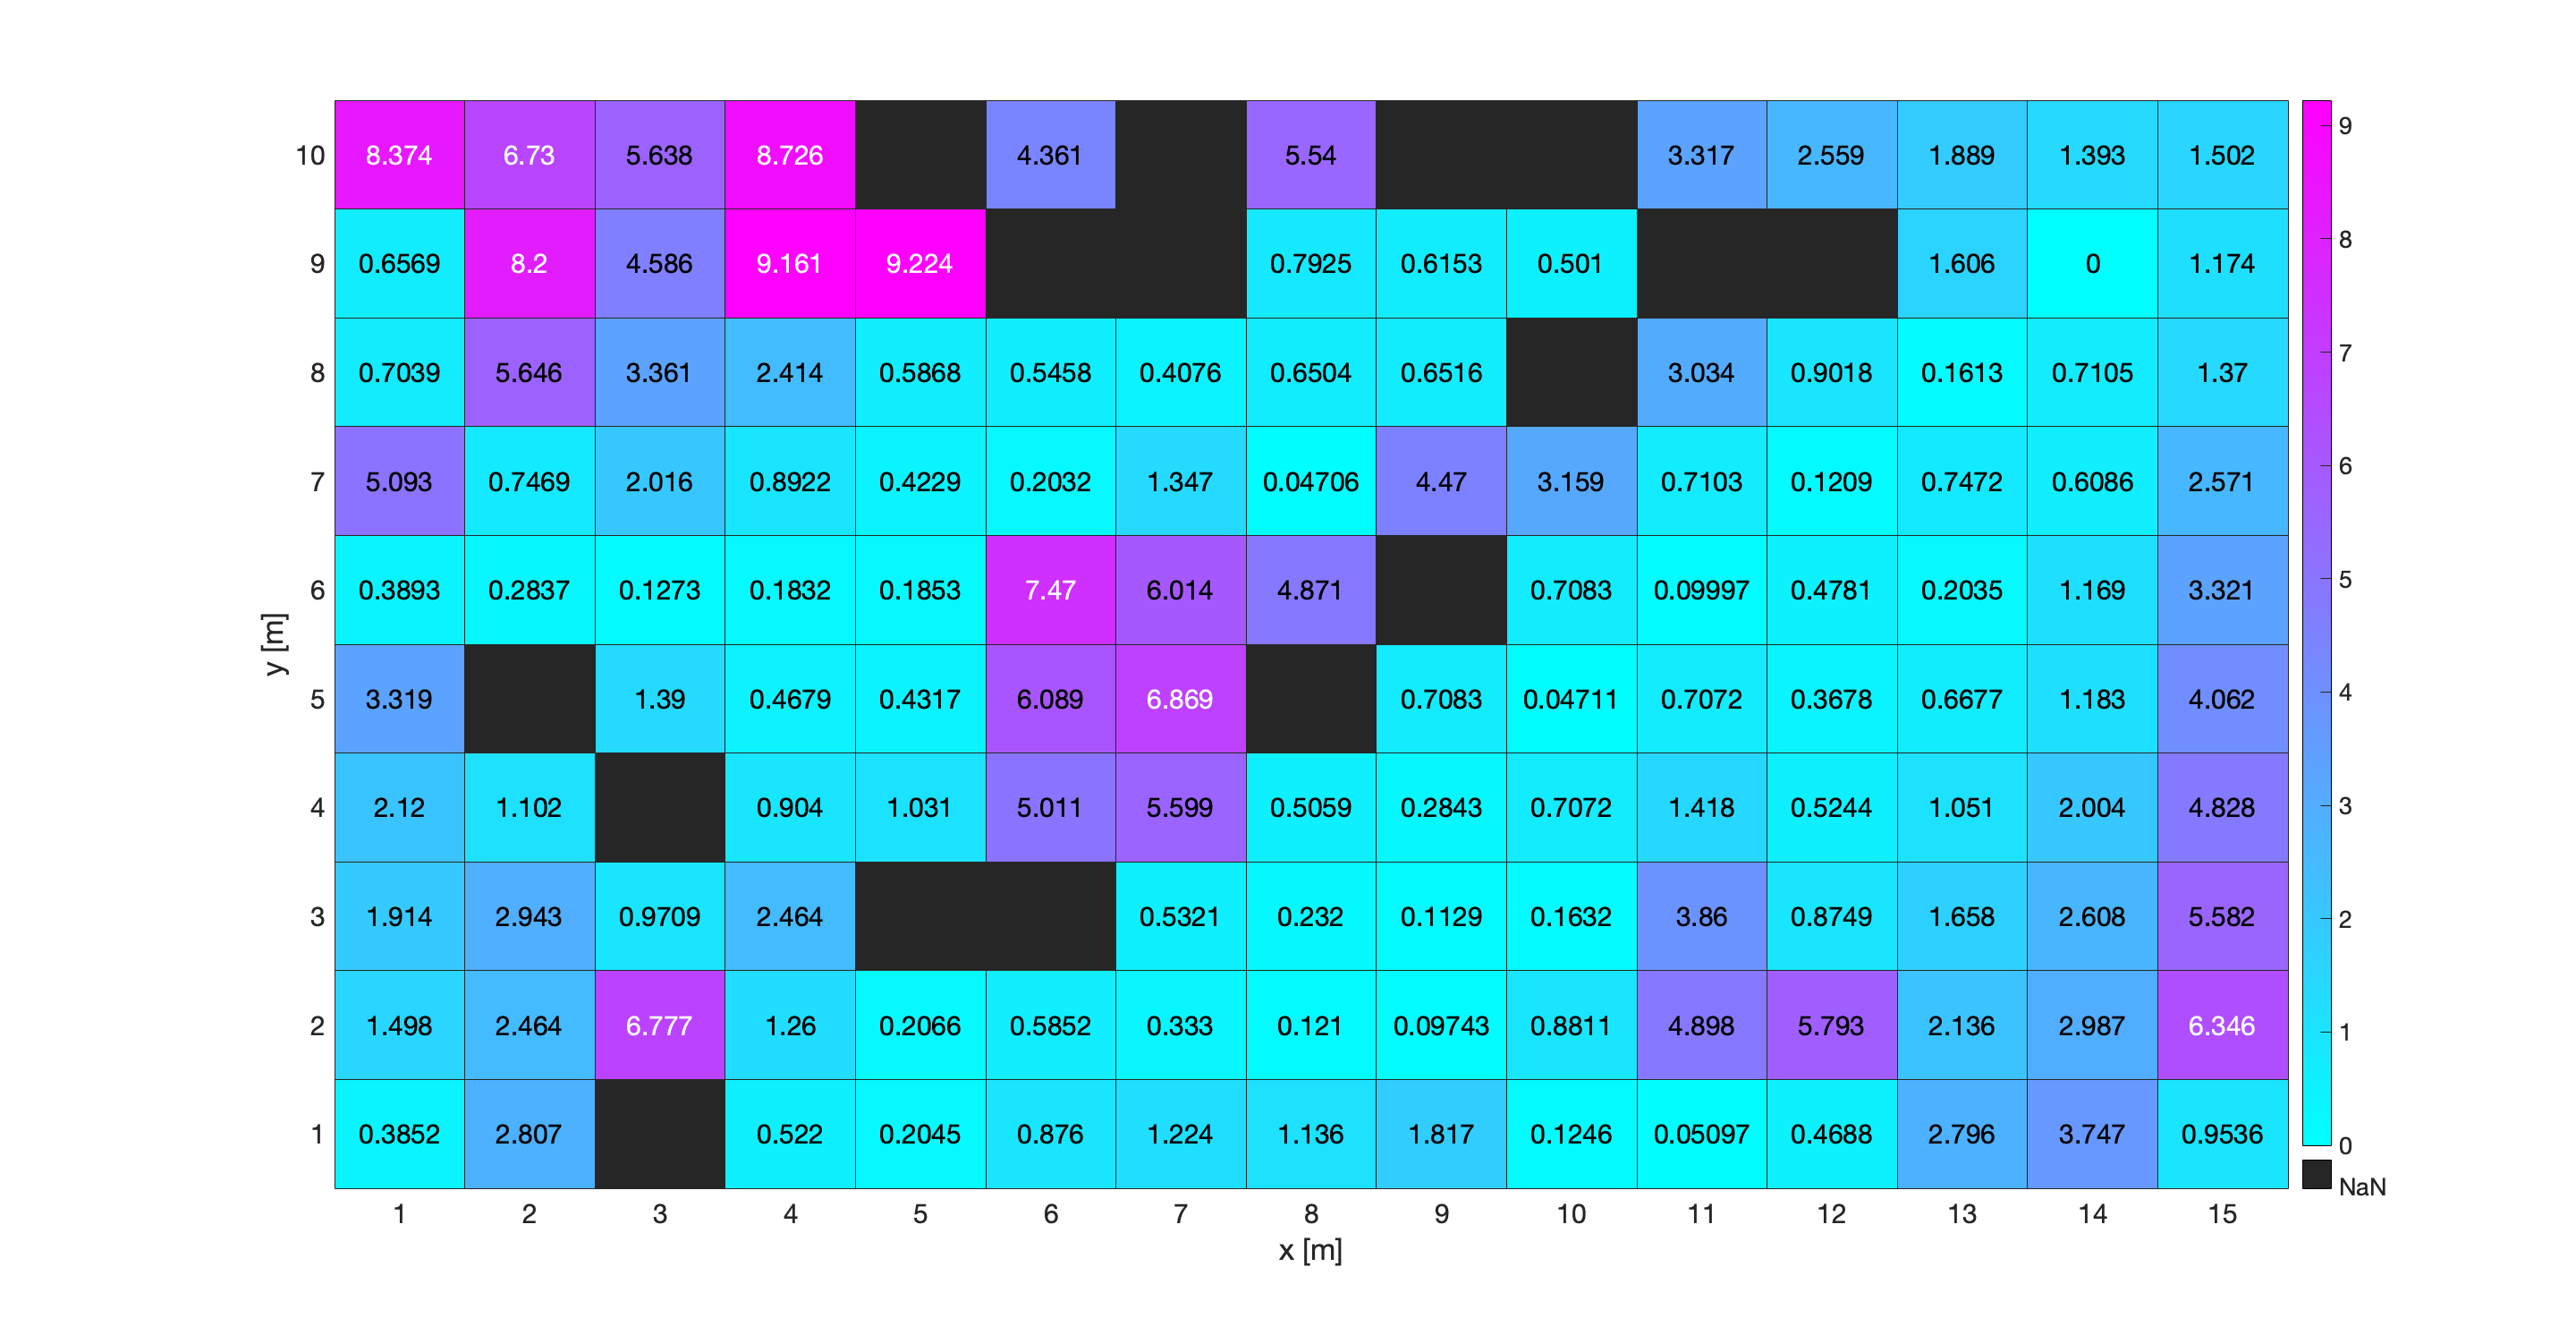
\includegraphics[width=.9\linewidth]{Images/hla_images/hla_anchor_(14_9)_clut.png}
\caption{Anchor located at (14, 9).}
\end{figure}

\begin{figure}[H]
\centering
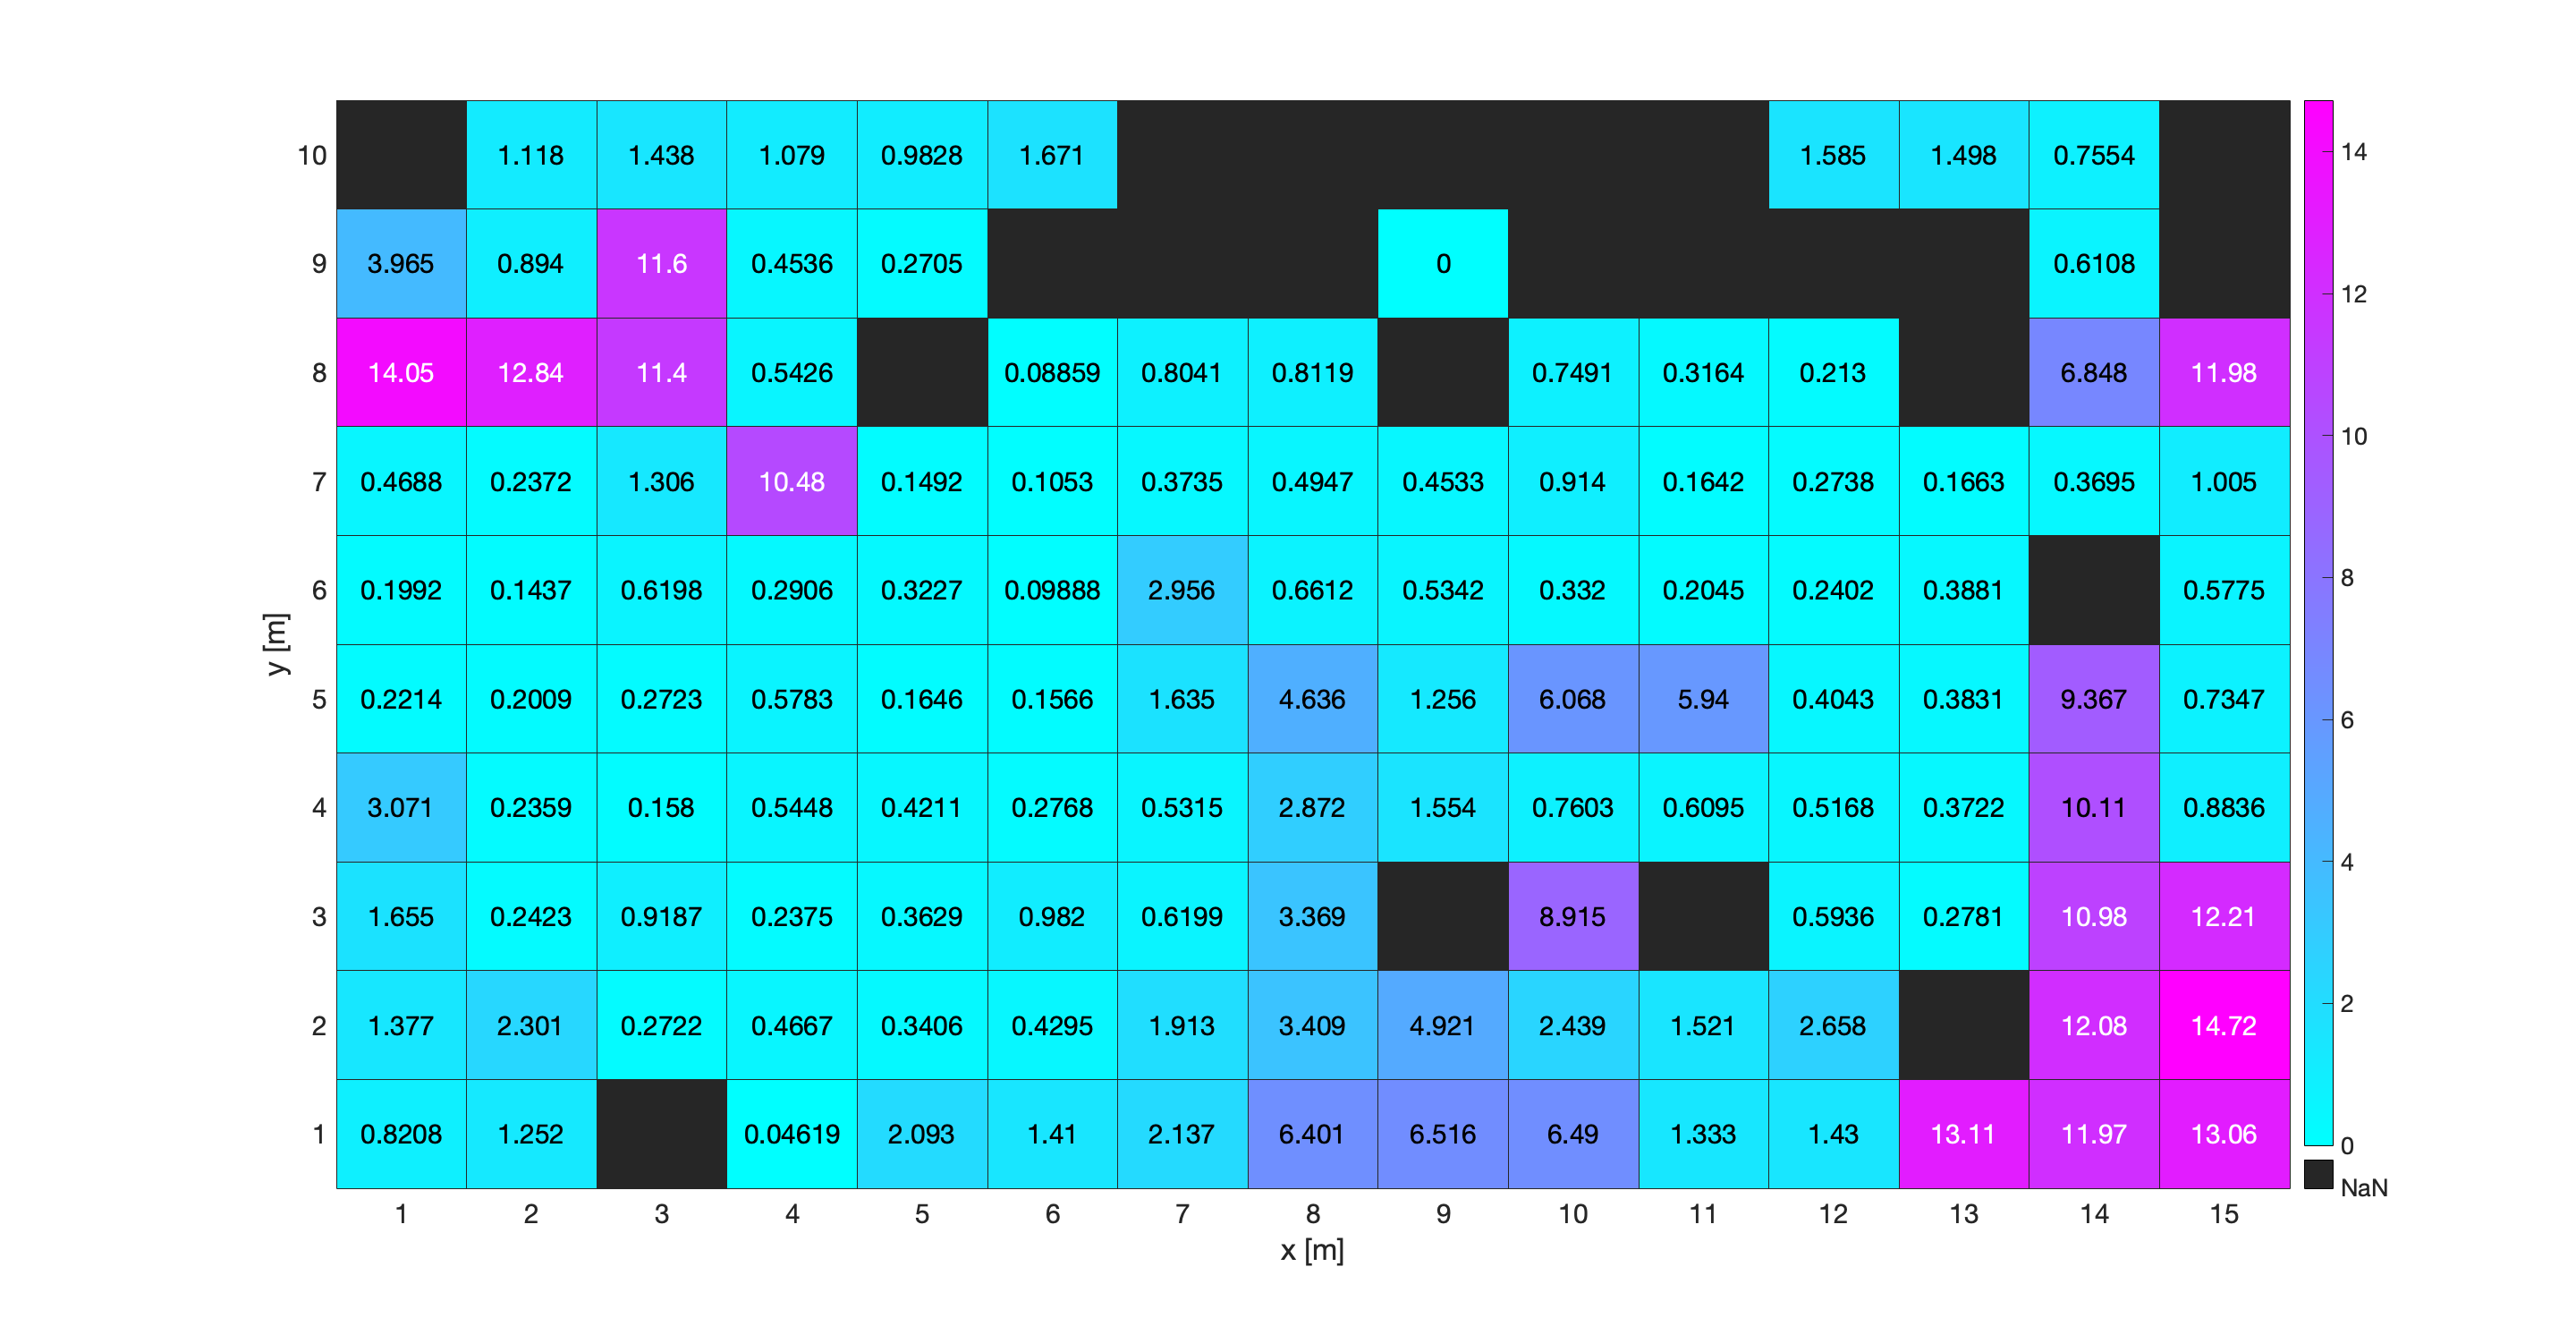
\includegraphics[width=.9\linewidth]{Images/hla_images/hla_anchor_(9_9)_clut.png}
\caption{Anchor located at (9, 9).}
\end{figure}

\begin{figure}[H]
\centering
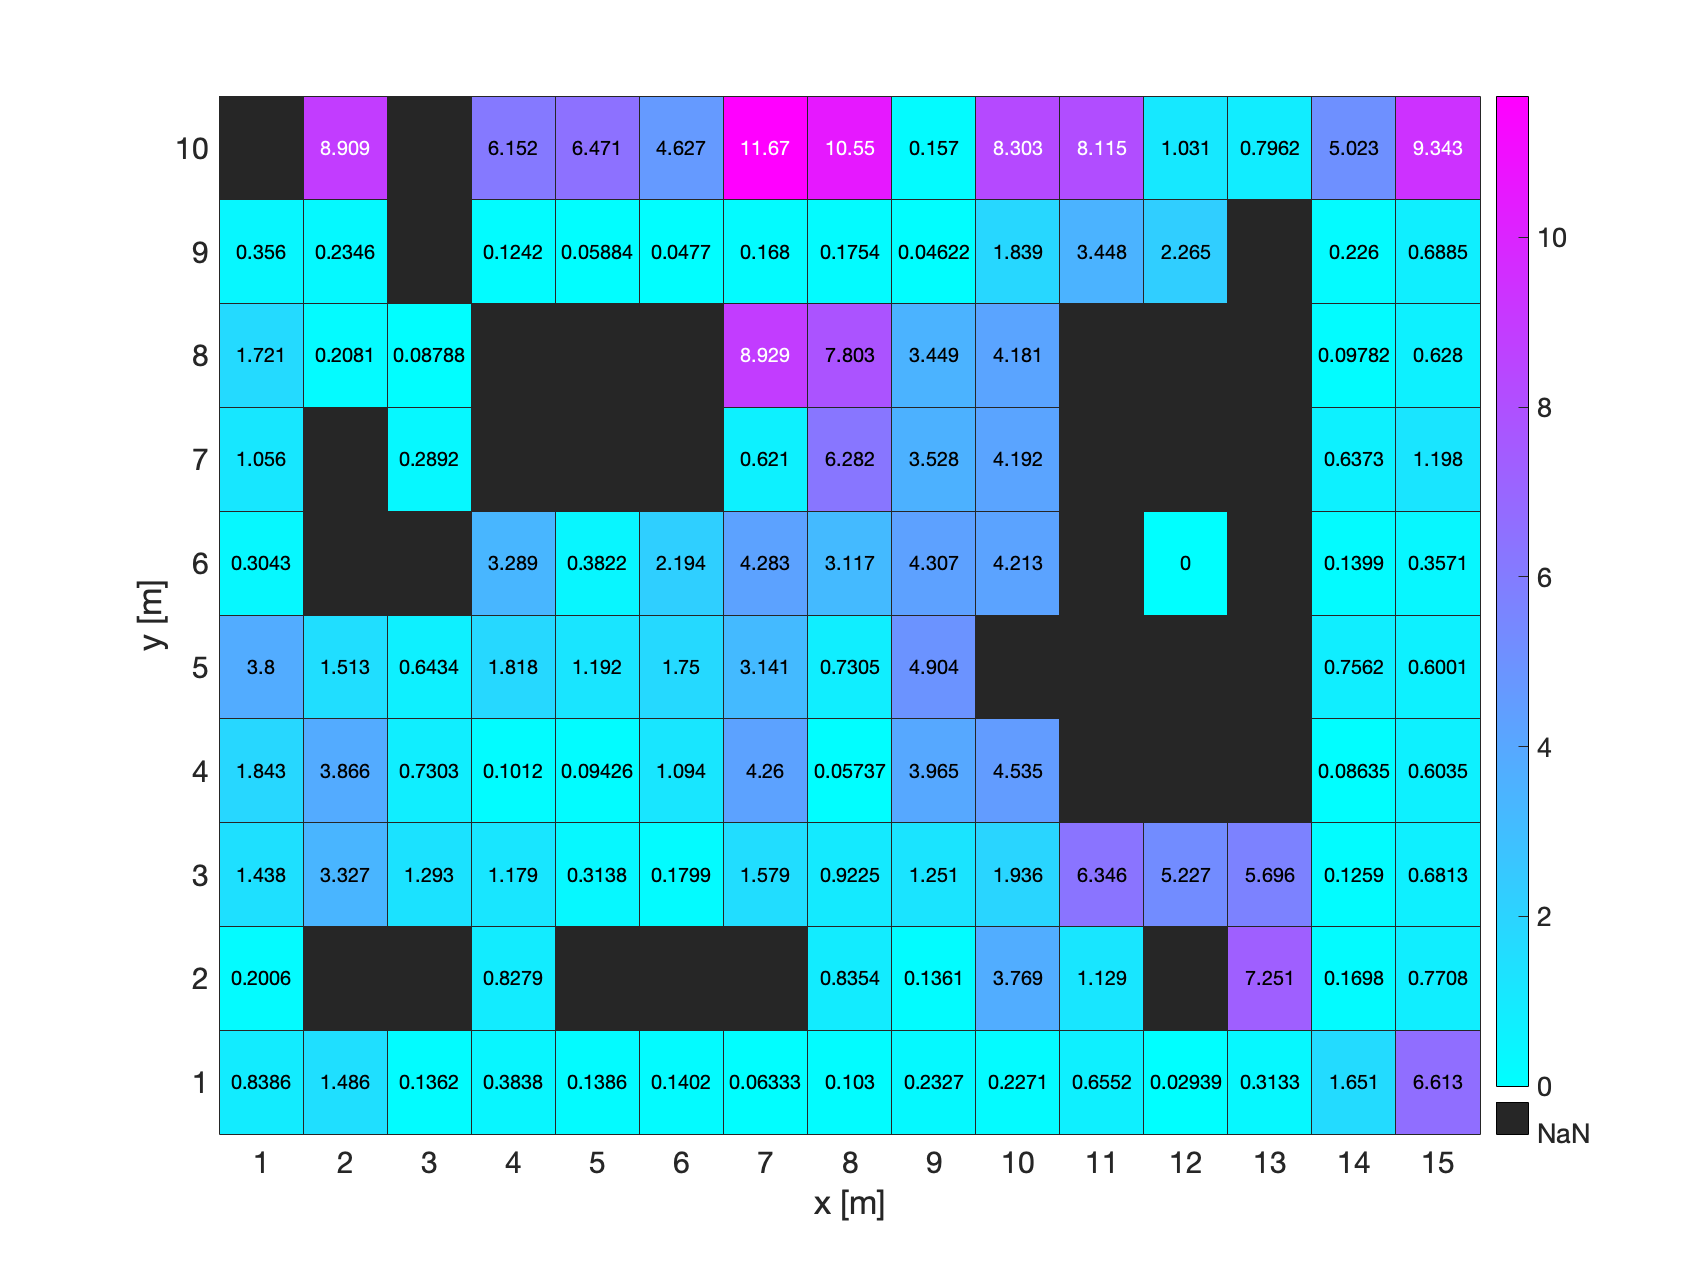
\includegraphics[width=.9\linewidth]{Images/hla_images/hla_anchor_(12_6)_clut.png}
\caption{Anchor located at (12, 6).}
\end{figure}

\begin{figure}[H]
\centering
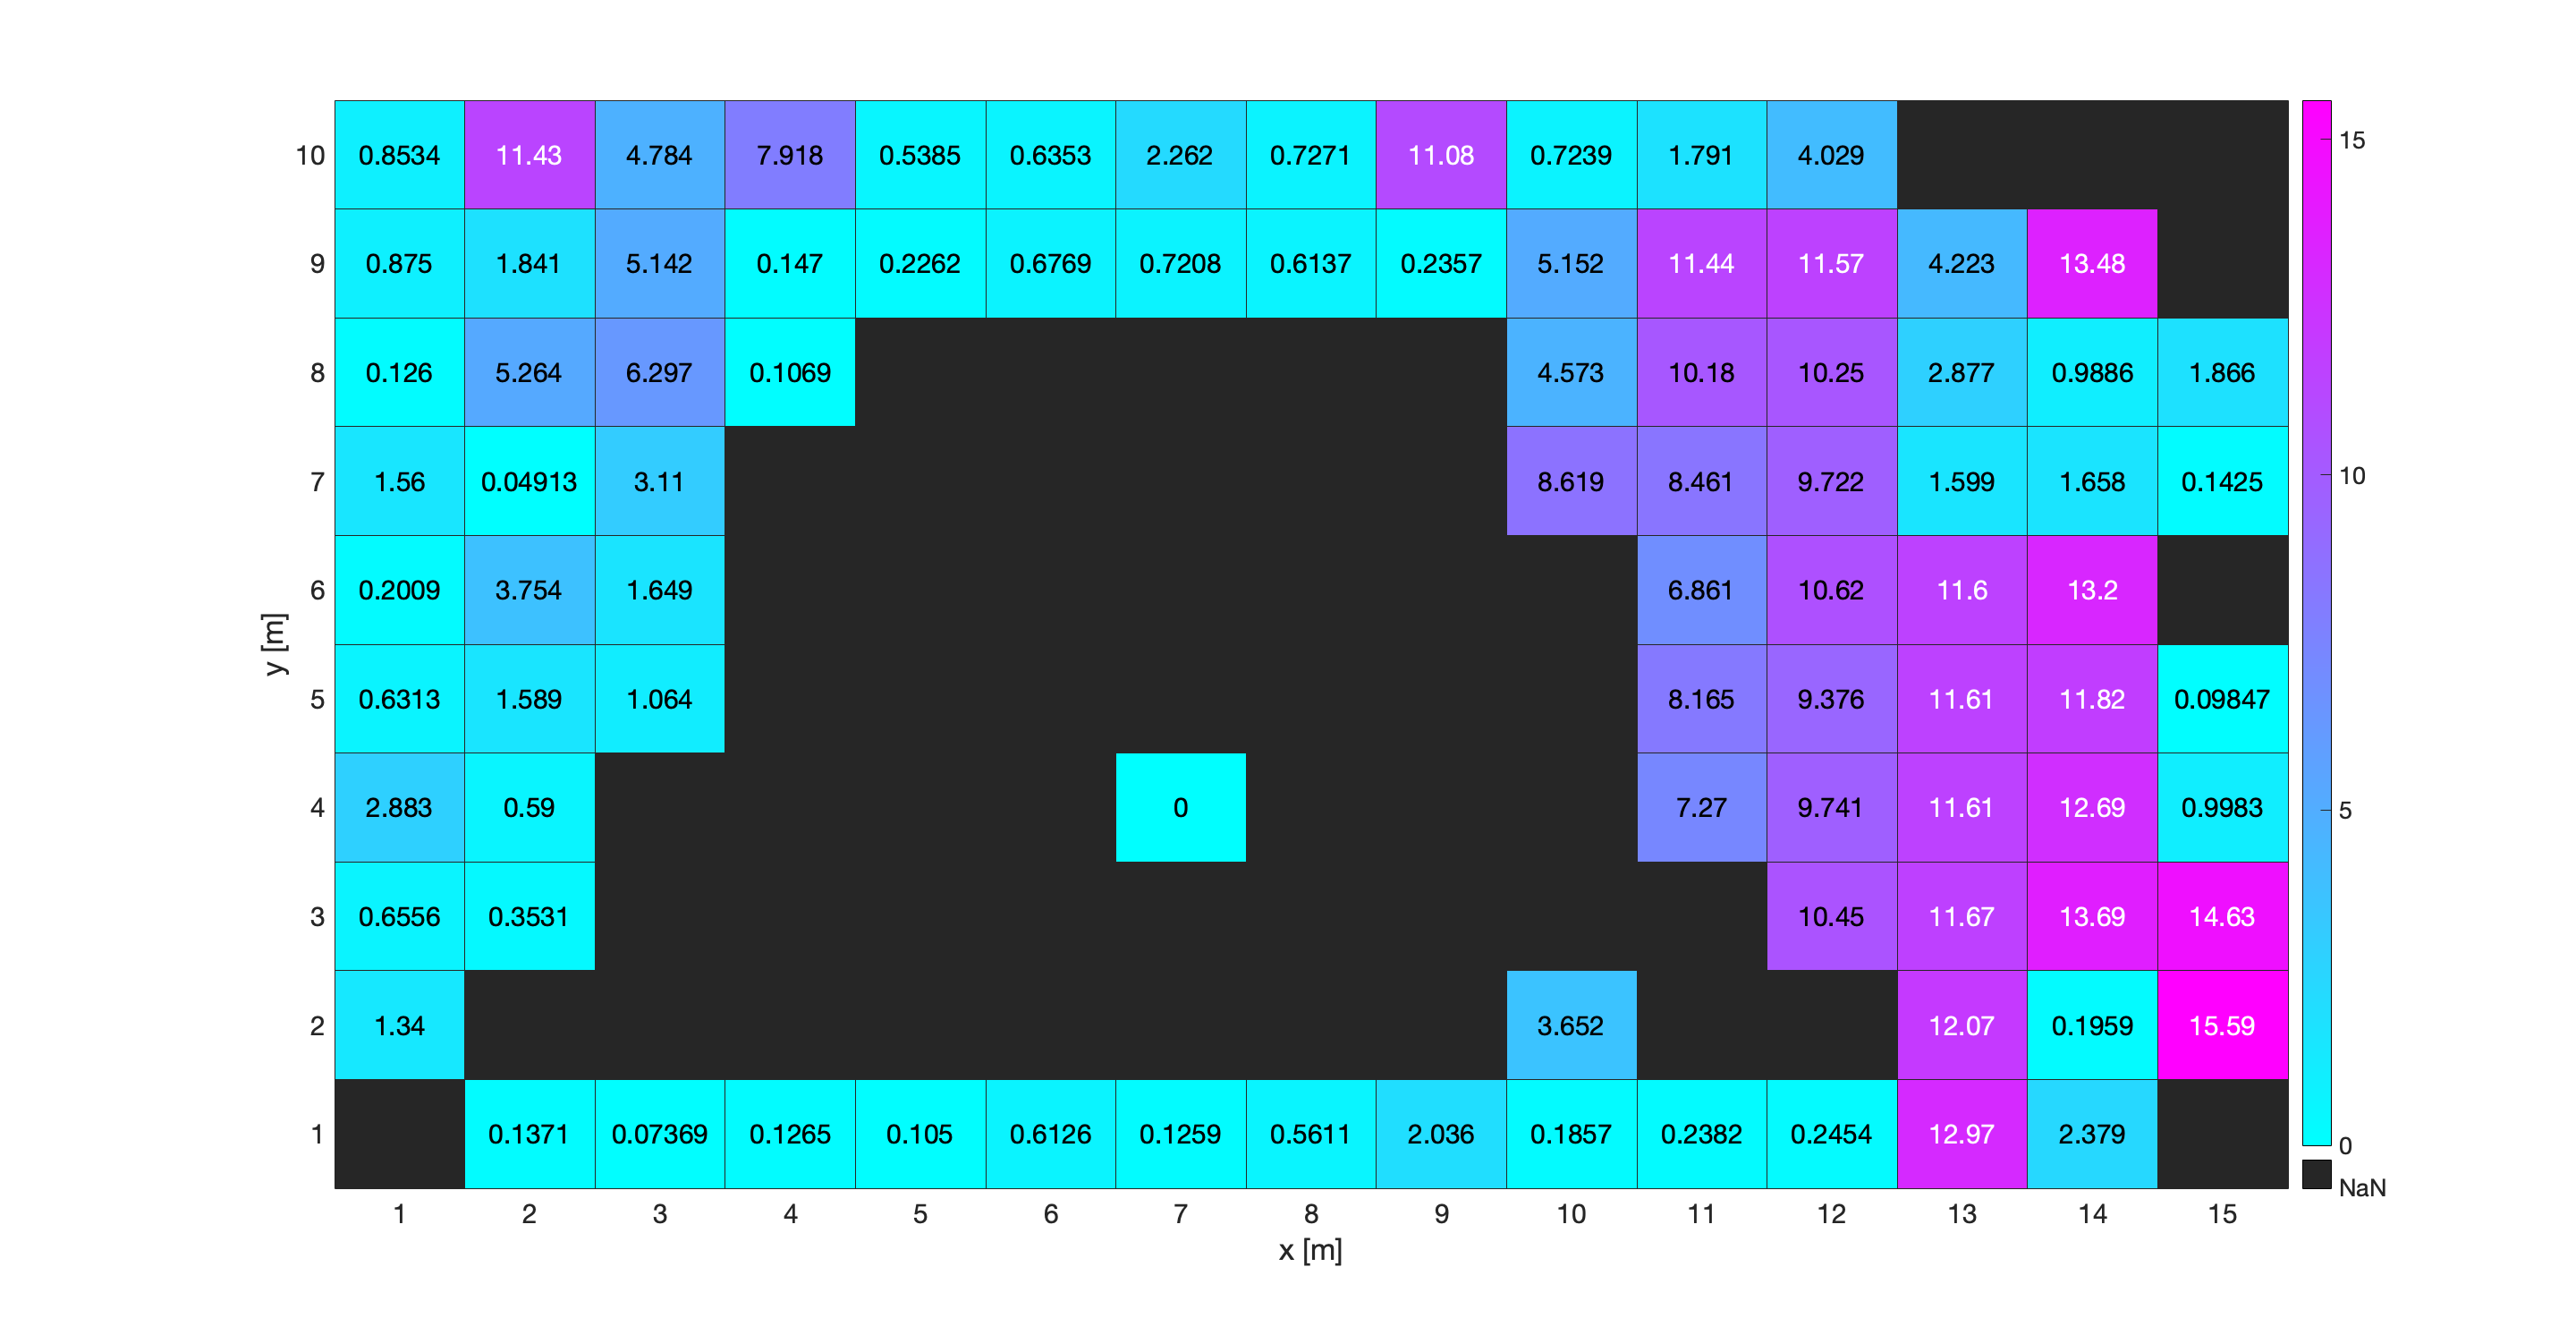
\includegraphics[width=.9\linewidth]{Images/hla_images/hla_anchor_(7_4)_clut.png}
\caption{Anchor located at (7, 4).}
\end{figure}

\begin{figure}[H]
\centering
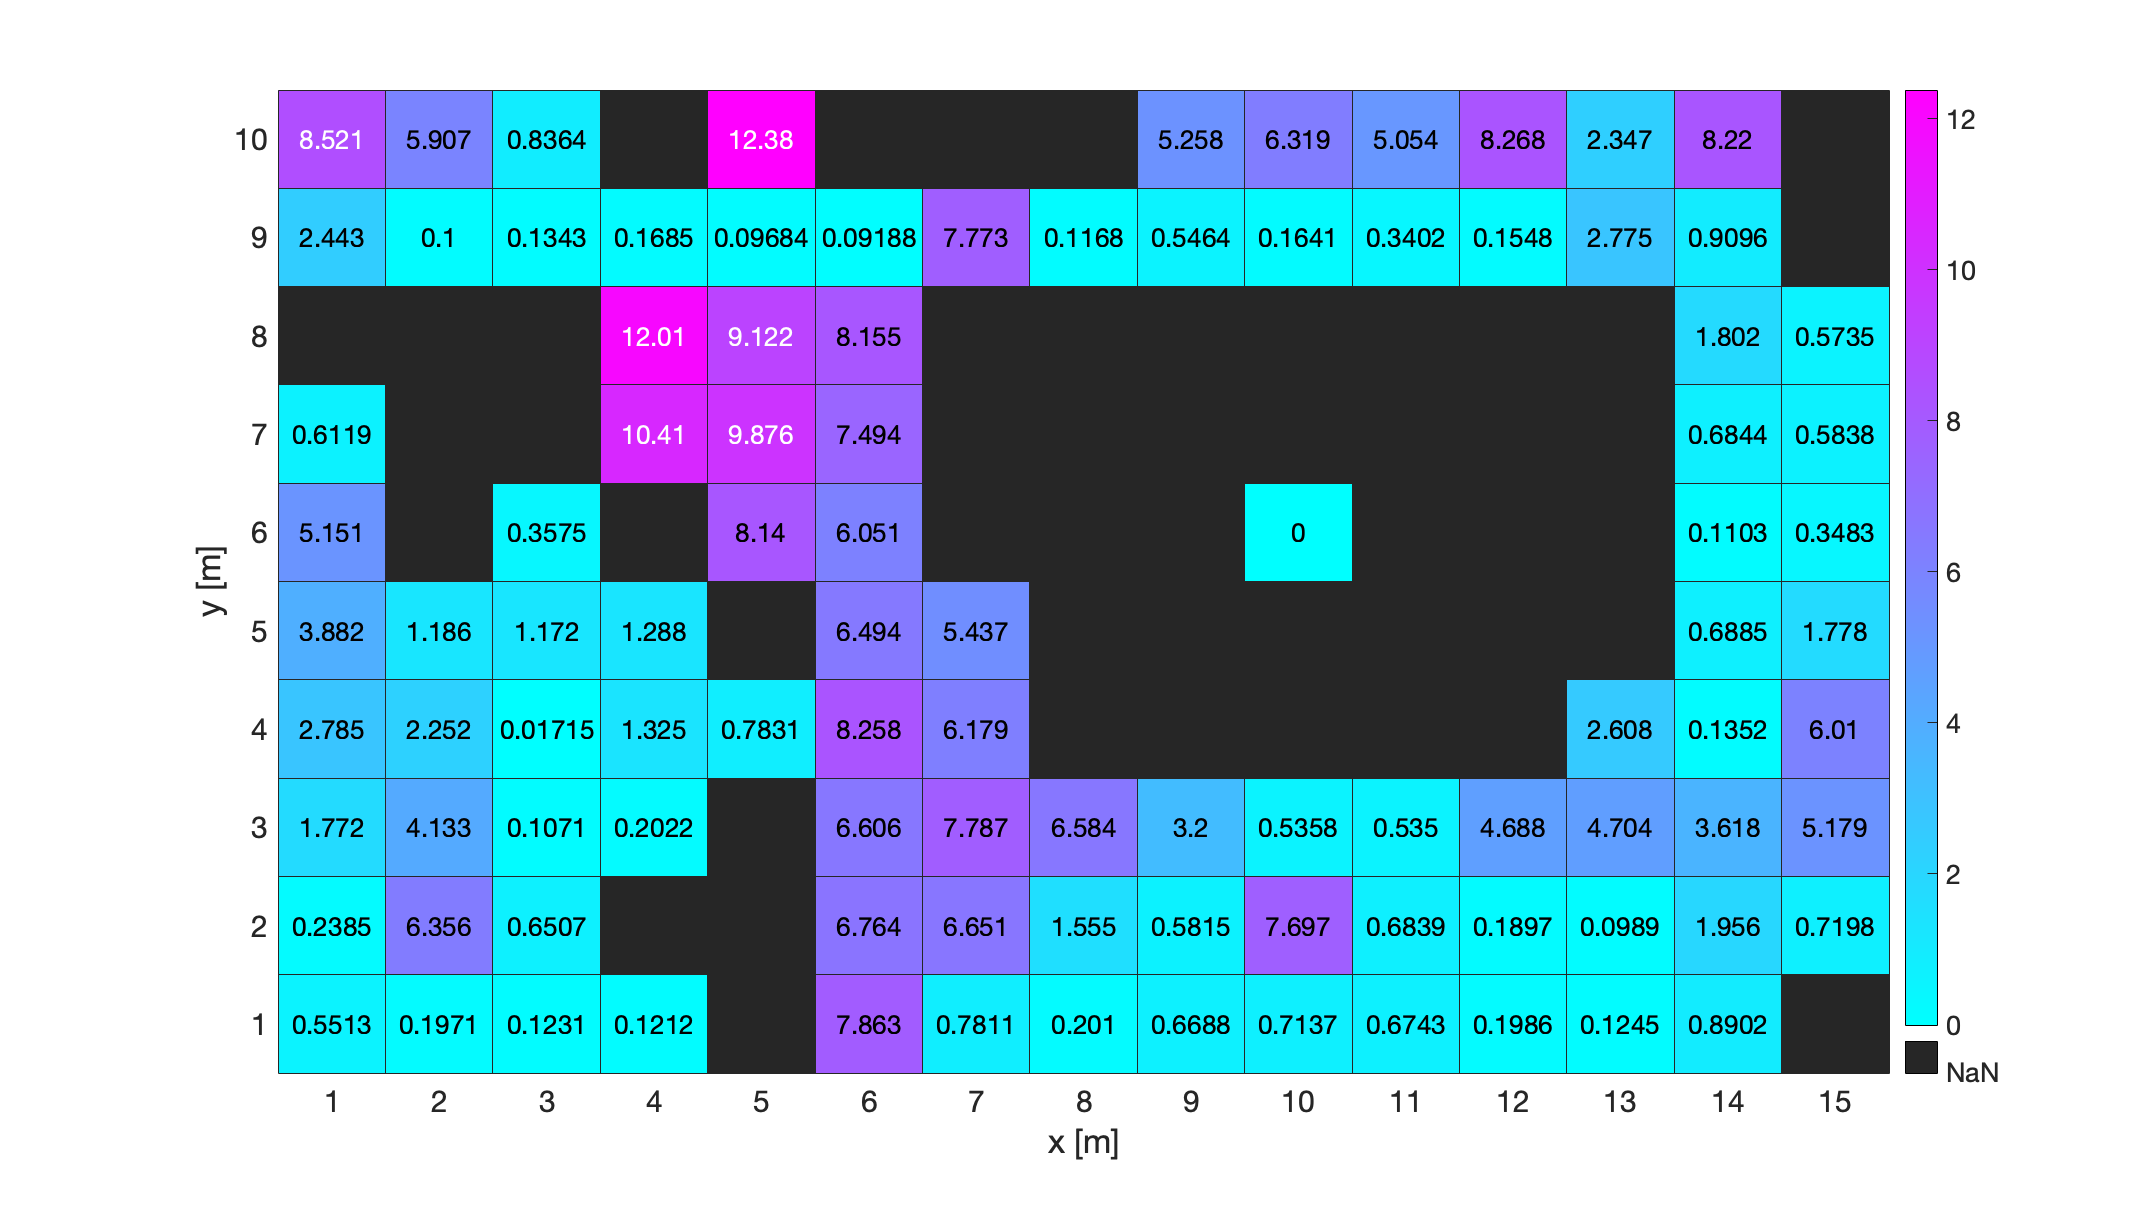
\includegraphics[width=.9\linewidth]{Images/hla_images/hla_anchor_(10_6)_clut.png}
\caption{Anchor located at (10, 6).}
\end{figure}